\section{Background and Previous Work} \label{sec:background_perious_work}

In this section, the previous work done in this application is reviewed. The need for dune crest-line detection has risen recently due to many research applications in this field. Therefore, understanding the concepts and properties of dune fields is important. 
%Section \ref{subsec:dune_pattern_studies} will present an overview of some of the research done in this field. Section \ref{subsec:image_processing_cv} will discuss some of the related algorithms and methods for processing images and computer vision used in this research. Finally, section \ref{subsec:dune_detection} will present the state of the art dune detection research which uses both appearance-based and machine learning approaches.

%\subsection{Dune Pattern Studies} \label{subsec:dune_pattern_studies}

Many studies have been done on the topic of dune fields, with the ultimate goal of understanding how dunes form, behave, and which factors contribute to the systems. In \cite{Kocurek_Ewing}, an explanation of how dune-field patterns emerge is proposed and the degree of complexity from the standpoint of self-organizing system is discussed. Dune patterns are classified into two basic categories: simple or complex. According to this paper, a simple pattern is defined as having a single pattern type. Complex patterns are said to potentially have multiple spatially superimposed pattern types. Simple patterns trend towards a better ordering, so long as the wind regime remains constant. Changes in the trend of wind pattern will cause reorientation. Complex patterns can then be interpreted as the superposition of many generations of wind regimes.

Complexity can be measured using pattern analysis, measuring parameters such as the crest length, orientation, spacing,	defect density, and other properties. These properties would be very useful information to extract for the dune detection. Finding crest-lines	can help us identify the patterns, extracting meaningful data such as junctions, terminations, mergers, linking, and other interesting processes explained in \cite{Kocurek_Ewing}.

In later work, \cite{Ewing_Peyret_Kocurek_Bourke} studied the dune field pattern formations on the north polar region of Mars. These dunes are thought to be mostly inactive, with relatively no movement over a period of 4 to 15 Martian years. The reason this region is interesting is because there are two nearly orthogonal crest-line orientations present in the region. This complex system of superposition of multiple patterns in this example showcases a set of \emph{primary} and \emph{secondary} crest-lines which would be valuable data to automatically segment. The \emph{primary}	dunes are the largest-scale dunes, extend over the entire length of the image set, and contain many \emph{Y} junctions, an indication of well-organized linear dunes. In contrast, \emph{secondary} dunes are rounded, have less defined features, and are perpendicular to the main primary crest-lines.

Other interesting features are the so-called \emph{Slipfaces}. These typically appear along the \emph{primary} crest-lines, in areas of intersection with the \emph{primary} and \emph{secondary} crest-lines. Another feature are the \emph{Wind Ripples}. The ripples are present on the surface of most dunes with the exception	of \emph{slipfaces}. To detect	these types of features, a higher resolution image is a required, as those types of features are very small compared to the scale of the \emph{primary} and \emph{secondary}	dunes. \emph{Interdune Areas} are features specific to the area studied in \cite{Ewing_Peyret_Kocurek_Bourke},	have a polygonal shape, and are indicative of ice.

The rest of the paper describes an in depth statistical analysis of the features to compute the flow fields and understand the geomorphic relationships which are present in the area. The paper \cite{Ewing_Peyret_Kocurek_Bourke} provides a lot of interesting and valuable information which can be used to understand the application of automatic dune detection. If these features can be extracted, it would be interesting to see if we can do a similar statistical analysis based on the results presented. The next step would be to retrieve the HiRISE dataset and their data or ground truth to compare.

In the most recent work, \cite{Multi_spatial_analysis_aeolian_dune_field_patterns} study the aeolian dune-fields at different scales. Scale is an important factor to consider because aeolian dune-fields patterns can vary over	a wide range of scales, both spatially and temporally. Being able to measure the change of scale over time is important in order to investigate the environmental conditions of the studied region. Aeolian	dunes are developed typically in transitions from sand patches, to proto-dunes, to dunes, to dune-field patterns. Complex dune patterns are usually a juxtaposition of simple dune patterns are multiple scales. To summarize, being able to detect the crest-lines and other types of features at multiple scales is invaluable.

In other related work, \cite{Application_spatial_cross_correlation_detection_submarine_dunes} studied the migration of submarine sand dunes. The dataset used in this paper includes digital terrain models (DTMs) retrieved from high-density multibeam echosounders (MBES) taken of submarine sand dunes along the coast of New Brunswick. In order to measure the migration of these types of dunes, the motion was measured by simply subtracting the DTMs from sequences over time. The implementation uses a simple cross-correlation to find similarities from one set to the next. From the correlation matches found, the migration vector can be computed. The migration data processing can extract the flow fields of the dunes.

The research presented above is only a subset of the work done, but provides very valuable information on how, why, and what dunes are. The next section will describe some of the state-of-the-art technology in the field of image processing and computer vision. 
 
%\subsection{Image Processing and Computer Vision} \label{subsec:image_processing_cv}

%The main goal of image processing is to enhance and improve the quality of images in order to improve the performance of feature extraction. Computer vision is a field in which information is extracted from images for the purpose of understanding the image to solve a problem for a given application.

%\subsubsection{Preprocessing}

%For this application, the satellite images of the dune fields need to be processed using various known processing methods. Filtering out noise in images is critical to extracting good crest-line candidates. There are many common filtering approaches used in image processing and computer vision applications. In this application, satellite images of sand dunes may include various amounts of noise. In order to improve the dune detection algorithms, the goal of filtering is to filter out the noise while preserving or enhancing the necessary features such as the crest-line edges. In \cite{Bilateral-filtering-gray-color-images}, the bilateral filter is proposed, which allows flat noisy regions to be filtered while preserving strong edges. Bilateral filtering	is a simple non-iterative algorithm for filtering out noise.

%Another key process is to normalize the illumination of the dune fields. Illumination normalization is a process in which the image illumination is made to be more evenly distributed across the image, to make the illumination invariant in conditions of varying lighting. This processing is most commonly used in face detection or recognition applications. In \cite{Illumination_normalization_based_on_2d_gaussian_model}, a Gaussian illumination model is used to stretch the contrasts of darker areas. The process involves using a Quadtree method to divide the image into sub regions to find dark areas. The areas that meet these requirements are processed with the Gaussian illumination model to brighten them up, which evens out the illumination. Applying this normalization significantly improves performance of face recognition.

%In a similar approach \cite{Illumination_normalization_for_image_restoration_using_modified_retinex_algorithm}, the authors use a modified retinex algorithm to restore poorly illuminated areas of an image. According to Lambertian reflectance theory, images consist of two components, reflectance and illumination. If an image contains a set of small scale features, and large scale features, and illumination is only applied to the large-scale set, then the small scale features can be preserved. In this approach, the normalization is applied to small-scale and large-scale features independently. The Single Scale Retinex process is applied to the image to separate	the reflectance (small scale) and illumination (large scale). After, images are thresholded and histogram equalization is applied, which spreads out intensity values of darker areas of the image.

%In a remote sensing application, \cite{Illumination_normalization_among_multiple_remote_senging_images}, illumination normalization is carried out in the gradient domain and using singular value equalization. According to the authors, the gradient domain image enhancement process can compress the dynamic range of images, increase contrast, and enhance fine details in darker regions. The goal of singular value equalization (SVE) is to make all images in a specific set to have similar mean intensity value. Some images may have a lower or higher mean intensity. By using SVE, the pixels can be processed to achieve a mean closer to the target intensity, therefore normalizing illumination accross a set of images. The drawback of this method is that multiple images of the same or similar scenes are required. Many of these techniques can be applied directly to processing the satellite images of the dune fields in order to improve and normalize the illumination.

%Another critical processing step is to extract edges from the images. Edges are extracted by taking the derivative of an image, and preserving the strongest gradients. There are many operators used to extract edges. The Canny edge detector, first introduced in \cite{1986_canny_edge_detection}, is a well known and used method to retrieve important edge features from an image. This famous detector is often used because of it's qualities in detecting edges. The Canny edge detector typically produces a binary image of thin, contiguous, and well defined edge segments which makes it a good candidate solution for edge extraction. 

%In \cite{Canny_edge_detection_enhancement_scale_multiplication}, enhancement to the method is proposed by analyzing the responses of detection at two scales. The benefits of this technique are better localization in images with larger amounts of noise, at the cost of a slightly lower detection rate. Overall the performance of the Canny operator is improved by using multiple scales.

%The Canny detector is further improved in \cite{Runway_detection_tracking_unmanned} for a runway detection application for unmanned aerial vehicles. The main contribution of this paper is the use the Canny operator combined with a mean filter, and using the Hough Transform to track runways. The advantages of the mean filtering is that it filters out noise, preserves edges (better than a traditional Gaussian filter), and makes the image less fuzzy. To solve the problem of the dual threshold of the Canny operator, the proposed method is to compute the thresholds dynamically based on averages.

%In \cite{Improved_Canny_Edge_Detection}, an improved implementation of the popular Canny edge detector is proposed. According to the authors, the traditional Canny algorithm suffers from two main	problems: the gradient calculation is sensitive to noise and the use of the fixed double threshold may not be suitable for images with high gradient variability. The main flaw in the gradient calculation has to do with the inequality of the edge detection in darker versus brighter regions. For the parameter selection of the double threshold, the paper propose choosing the high and low thresholds from the computed mean and standard deviation of the gradient magnitudes.

%Another problem with edge detection methods can be the discontinuity of edges. The goal is often to link edges which may suffer from noisy conditions in order to produce smoother contiguous segments. In \cite{Edge_linking_using_geodesic_distance_neighborhood_information}, an edge linking approach is proposed which using local neighborhood, using geodesic distance (as opposed to the common Euclidean distance measure) between edge candidates. When calculating the direction of edge end points, typically eight directions are used, which introduces error. To address this, \cite{Edge_linking_using_geodesic_distance_neighborhood_information} define a windows size based on the maximum allowable edge gap, and fit a line to the edges, which allows a full range of directions to be accounted for. The geodesic distance measurement is not only based on euclidean distance but also on the intensity values of the image, which reportedly gives better results.

%\subsubsection{Feature Detection}

%Once edges have been detected, the next logical step is to extract information from the edges. In previous work, in order to detect dune crest-lines, the edges needed to be organized into line segments so geomorphological properties can be computed. Computing the orientation and dune spacing of the dune field on the satellite images requires an algorithm that can accurately detect line segments present in an image.

%Line detection is a well known and challenging problem in the field of computer vision. Traditional approaches such the Hough Transform presented in \cite{1972_hough_transform_line_detect}, use edge detectors such as the Canny to extract line segments. Unfortunately, choosing the correct parameter and an appropriate threshold for preserving true positives while eliminating false positives for any task can be difficult. Inappropriate selection of the parameters causes inaccurate results in the computation of the geomorphological properties. Improvements on the technique proposed in \cite{1986_extracting_straight_lines} and \cite{2000_meaningful_alignments} improve the results slightly but basically suffer from the same parameter selection problems.

%An interesting alternative to the classical Hough transform is presented in \cite{Automated_cable_tracking_sonar_imagery} in an application inspection or maintenance of underwater cable components. The paper discusses image processing techniques to extract linear features in cluttered and noisy images. After applying some anisotropic filtering to remote high frequency noise, edges and lines are detected on the sonar based images. To detect potential linear features, they use a Phase Congruency detector. The Hough transform is then used to find linear features, and a criteria is determined to reject false positives and preserve true positives.

Another promising approach to line segment detection is presented in \cite{2010_lsd_fast_line_segment_detector} which combines the features of the techniques presented above. In this approach, adjacent edge points are group by orientation, and lines are fitted to the local support region. Validation of line segments is applied using a threshold of the number of points which support the given line. The benefits of this approach is the ability to detect line segments in complex structures using minimal parameter selection. 

\begin{figure}
	\centering
	%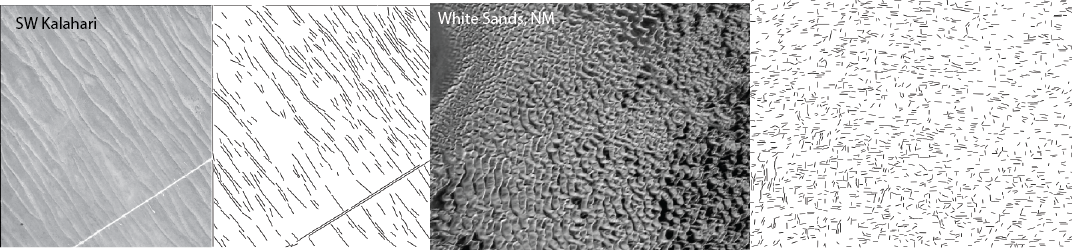
\includegraphics[width=\linewidth]{figures/lsd_results}
	\caption{Preliminary results of the Line Segment Detector (LSD \cite{2010_lsd_fast_line_segment_detector}) applied to the linear dunes of the Kalahari (left) and transverse dunes in White Sands (right). The results of the LSD on linear dunes are good, while complex transverse dune results are poor.}
	\label{fig:lsd_results}
\end{figure}

Some preliminary work was done testing the Line Segment Detector (LSD) on some dune field images, shown in Figure \ref{fig:lsd_results}. The method seemed to perform quite well on linear dune formations found in regions like the Kalahari, but performance was quite poor on regions with non-linear complex or transverse dune formations, such as the White Sands dune field.

A line detection and image enhancement has also been proposed in \cite{Robust_Faint_Line_Detection_Enhancement_Algorithm}, for a digital image restoration of heritage artwork. The images worked with have been deteriorated over time, and contain many cracks, faint lines, and broken stroke. The goal of this is to remove unwanted edges, and enhance the desired edges. The approach is implemented in three basic steps: Initial line detection with non-maxima suppression, true line detection using anisotropic refinement, and noise reduction. The initial step is to perform correlation convolving the image with some sort of edge detecting mask, rotated at different orientations, and retrieving the maximum response for the orientation	for each pixel. The paper claims this produces a sharper and more reliable edge map, which is then filtered using non-maxima suppression. This process preserves strong lines while removing texture lines. The image is the binarized to remove all remaining weak edges, and only allowing strong edges to remain. The smoothing is applied to the original based on the processing done, smoothing out weak edges, while not smoothing strong true edges.

%In a similar approach, \cite{Image_Edge_detection_Rotating_Kernel_Transformation} use rotating edge detection kernels and fuse the responses from the operations. An edge is defined as a location and a direction compared to a non-edge point such as a flat area or noise, which has no specific direction. Following this principle, the response in one direction should be higher than in the other directions. For a non-edge, the	responses in each of the directions are similar. Therefore computing the mean and standard deviation of each of the kernel responses can help resolve edge versus non edge pixels. The results obtained from this process shows promising results when applied to noisy images. The approach proposed in \cite{Image_Edge_detection_Rotating_Kernel_Transformation} has definite potential for improved edge detection applied to dune crest-line detection. It also has potential for improvement of the method itself.

\begin{figure}
	\centering
	\begin{subfigure}{0.35\textwidth}
		\centering
		%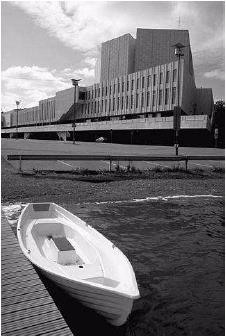
\includegraphics[width=\linewidth]{figures/tensor_voting_input}
		\caption{ Sample Image }
		\label{fig:tensor_voting_input}
	\end{subfigure}
	\begin{subfigure}{0.35\textwidth}
		\centering
		%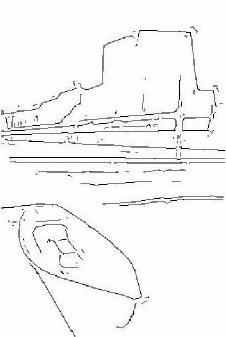
\includegraphics[width=\linewidth]{figures/tensor_voting}
		\caption{ Tensor Voting Results }
		\label{fig:tensor_voting_output}
	\end{subfigure}
	\caption{ The results of applying tensor voting schemes to find salient linear segments in an image (\cite{2009_tensor_voting_cluttered_backgrounds}) }
	\label{fig:tensor_voting_results}
\end{figure}

Tensor voting frameworks are also a potential way to extract linear segments from images, and could be useful in a dune detection application. Tensor voting has been used in various applications in computer vision such as in \cite{2006_tensor_voting_video_repairing,2005_tensor_voting_image_correction,2006_tensor_voting_stereo_monocular,2005_tensor_voting_visual_motion_analysis,2001_tensor_voting_epipolar_geometry}. One of the interesting benefits of tensor voting approaches, as explained \cite{2009_tensor_voting_cluttered_backgrounds}, is that they seem to show very good results in grouping oriented segments in highly cluttered images. The Gestalt principles of visual perception are used as the voting scheme where second order tensors are used to represent the segments. The goal is to filter out background segments while preserving the more salient segments. Figure \ref{fig:tensor_voting_results} shows the result of applying tensor voting to a sample image.

%In \cite{Probabilistic-tensor-voting-robust-perceptual-grouping}, a tensor voting approach is used to perform perceptual grouping on noisy data. The approach extends the standard tensor voting using Bayesian probabilities. The Bayesian framework has added benefits of	reducing the learning variance of the perceptual grouping task. Another	contribution of this paper is the use of a 2\textsuperscript{nd} order tensor and two	types of polarity vectors to handle both outliers and inlier noise. The approach also is able to process all types of geometric structures. For probabilistic tensor voting, the voting procedure uses random vector with a given standard deviation. It uses three layers of voting:	sparse ball vote, sparse stick vote, and revised stick vote, where the goal is to change the positions of each token based on a random vector.

%Another interesting approach for extracting features is segmentation. One particular method used in segmentation processes is the Watershed Transform, an approach which is used in this research and explained in section \ref{subsec:watershed_transform_segmentation_approach}. The Watershed Transform is a well known algorithm for segmenting meaningful regions from an image. The main benefit of the watershed technique as opposed to methods, such as edge-based detection, is that the watershed produces closed boundaries, which allows contours to be detected. An overview of the Watershed algorithm	is presented in \cite{Watershed-transform-definition-algorithms-parallelization-strategies}.

%In \cite{Image_segmentation_using_texture_gradient_based_watershed_transform}, segmentation is achieved using the watershed transform from texture gradients. The texture gradients are retrieved using various wavelet transforms. Similarly, in \cite{Watershed-based-textural-image-segmentation}, an approach to texture segmentation is proposed. When applied to textures,	the watershed algorithm tends to over-segment a texture into small homogeneous sub-texture regions. Therefore, a texture can be determined	to be set of texture segments. The texture sub-regions can be merged using a clustering algorithm. A wavelet transform is used to characterize the irregular shaped segment regions, which are used to cluster similar	groups of sub-textures.

%Another approach used in the Watershed algorithm is based on markers. The desired regions to segment can be extracted using some known feature which is marked on the image. In \cite{Fingerprint-pore-extraction-based-marker-controlled-watershed-segmentation}, this concept is applied to fingerprint pore extraction. Marker based segmentation has been shown to be robust for segmentations problems where the objects are closed contours with boundaries being ridges. In this application, the watershed transform is applied to the gradient image of the fingerprints, and the regional minimas are computed to obtain the markers, then compute the watershed transform based on the markers. In \cite{Detection-breast-tumor-candidates-using-marker-controlled-watershed-segmentation}, the watershed segmentation is applied to a breast tumor detection application. All these various researches have the potential to be useful in our dune crest-line detection application. 

%Ultimately, the goal is to perform automated feature detection from satellite images. In \cite{Extraction_roads_multispectral_imagery}, a semi-automated method for extracting roads from aerial or satellite images is proposed. The purpose of this paper is to localize roads from higher resolution images, using some form of segmentation. The proposed method is semi-automated because a user must provide and initial seed point, onto which a region growing algorithm is applied to extract the road. A level set method is applied to evolve the boundary of the road region, which can better handle noise and multiple road mergers. The boundary for the desired region is based on a speed function, which is designed based on uniformity, texture, and contrast properties. Once the regions have been extracted, the centerlines of the roads are estimated using a skeletonization procedure, with junction analysis to ensure that intersections are properly handled.

%In \cite{Extracting_ocean_surface_feature_modis}, linear features of internal waves are extracted using a technique called \emph{Multiscale Retinex}(MSR) feature extraction. Although the problem set in \cite{Extracting_ocean_surface_feature_modis} is different, there appears to be significant overlap and comparison between dune crest-line detection and oceanic internal wave detection. The oceanic internal waves are typically generated from many sources such as tidal currents, ocean frontal boundaries, and other atmospheric conditions. The MSR is an image processing technique that provides consistency and dynamic range compression across an image with poor contrast. The paper discusses the use both the Wavelet Transform Modulus Maxima (WTMM) and the Canny edge detector, which turned out to have superior performance.

%\subsection{Dune Detection} \label{subsec:dune_detection}
The specific application of this research applies to automated detection of dune crest-lines. Some work has been done in automated dune detection. There are two main methods used to detect dune landforms and crest-lines: appearance-based and machine learning methods.

%\subsubsection{Appearance-Based Methods}
In \cite{2012_automated_extraction_sand_dunes_egypt}, a Geographic Information System (GIS, \cite{gis_article}) based model is proposed and developed to study sand dune migration patterns, with the ultimate goal of predicting threats to roads, irrigation networks, water resources, urban ares, agriculture and infrastructures. Multi-temporal images of a region were collected, enhanced, and a simple image subtraction technique is used to compute the migration shift of dunes.

An automated extraction of dune features approach is proposed in \cite{2015_automated_mapping_of_linear_dunefield}, which uses the Sobel gradient operator to detect crest-lines. In this approach, the authors claim that the Canny edge detector provided poor results, and the Sobel operator generated more consistent results. The gradient magnitude of the Sobel operator is used to threshold out the weaker edges. The use of a histogram to compute the orientations of the gradients was found to have a bimodal distribution, with one of the modes being the dune edges. Dune candidates are determined based on their gradient magnitude which filter out weaker candidates unless they are near strong candidates. This research addresses the issue of determining crest-lines versus valleys or shadows, explained in section \ref{subsec:challenges}, by using the histogram of gradients. Examination of the histogram reveals that they had a strongly bimodal distribution for which one peak represents crest-lines and the other represents the valleys or shadows. The assumption made in their research is that the stronger peak represents the crest-lines, and therefore all gradients which belong to the weaker peak (within 90 degrees of the peak) are filtered out. This assumption may not always be valid, and is addressed in section \ref{subsec:edge_based_detection}.

In \cite{2016_comparisons_crest_line_extraction_marine_dunes}, an overview of various line detection algorithms are reviewed in the context of a marine dune crest-line extraction method. The research evaluates four main appearance-based approaches (\cite{2005_topology_driven_algorithms_for_ridge_extraction,2005_smooth_feature_lines_surface_meshes,2004_ridge_valley_lines_meshes_surface_fitting}) to detecting ridges from MultiBeam Echo-sounder System (MBES) data maps. The data for these approaches is essentially 3D depth maps of underwater dune forms. The challenge therefore is to trace the ridges to extract the dune crest-lines.

%\subsubsection{Machine Learning Methods}
Many of the research techniques to detect and identify various landforms use commonly known machine learning techniques. In \cite{2006_automated_classification_landform_elements}, object-orientated image analysis is used to classify the type of landform elements found in Digital Terrain Models (DTM). Features such as elevation, curvature, and slope gradient are used to construct a classification model, which categorizes landform elements into nine distinct base shapes. The shapes are somewhat abstract and generalized, but the concepts presented in this paper could be applied to crest-line detection.

The research done in \cite{2007_Machine_Learning_tools_automatic_mapping_mars} developed a machine learning based approach to map and categorize various landforms on Mars. In this research, it is shown that regions can be clustered using unsupervised learning methods, and labeled using supervised learning, given a dataset which has been manually labeled. The popular Support Vector Machines classifier is used to predict the label of the clustered regions. Similar methods will be addressed in sections \ref{subsec:edge_based_detection}, \ref{subsec:machine_learning_approach}, and \ref{subsec:mixed_ml_gradient_approach}.

The research done in \cite{2013_sar_image_automated_detection_dune_area} uses a simple approach in which the correlation is computed between two images taken at different times within a year. Various window sizes are used to account for dunes of different scale. An interesting observation is made; as the window size grows larger, the correlation values tend to increase in areas where dunes are present, while remaining relatively constant in areas without dunes. A supervised learning method is used to classify areas which dunes are present.

In \cite{BandeiraMarques}, a supervised learning approach is used, training classifiers such as Support Vector Machine and Random Forests to detect dune structures on Mars. The method proposed in this paper is to classify small (40 by 40 pixels) cells in a quantized image grid. In each cell, features are computed based on the image gradients, using both phase and magnitude. In order to classify a cell as either a dune or not a dune, the features of both the cell and the cell's neighboring cells are used. The features extracted are then used to train the machine learning method, which is used to then predict if a cell is a dune.

Although this type of method has typically shown very good results, there are a few drawbacks with using supervised learning approaches. These types of methods usually require a fairly large labeled dataset which may not always be available. Anytime a dataset is constructed for this purpose, it is important to provide a large number of examples of different types of dunes, in order to get a robust representation of the problem set. In \cite{BandeiraMarques}, 230 labeled images were used to train and test the method, and have a decent representation of various dune types. Another drawback of this approach is the use of cells, for which fixed-sized cells may not be scale invariant. Also, quantizing an image into larger cells	will affect localization accuracy of the dunes. If the application requires higher localization accuracy, this type of supervised learning approach may not be suitable.

In \cite{2011_neural_network_based_dunal_landform_mapping}, texture features are extracted from images to train a multilayer perception or neural network to generate landform maps. The texture features used are the Grey Level Co-occurrence Matrix (GLCM \cite{1973_textural_features_image_classification}), are fed into the neural network with goal of characterizing various landforms. A critical problem to solve is the selection of the window size for computing the texture features. Reportedly, smaller window sizes, relative to the spatial resolution, negatively affect the classification accuracy. The window size parameter is also addressed in section \ref{subsec:machine_learning_approach}. A large dataset was used to train the neural network, and shows promising results.

The most current and direct research application to dune crest-line detection is presented in \cite{vaz_object_based_dune_analysis}. An object-based image analysis method is used to extract crest-lines from dune field datasets on mars. The main approach extracts features from the dune field images, and trains an artificial neural network classifier. Once the classifier is trained, the crest-lines can be extracted and the dune field can be analyzed. The object-based image analysis methodology is very similar to our research, and the datasets used in this paper were acquired. Section \ref{subsec:results-and-discussion} shows the comparison of the results reported in \cite{vaz_object_based_dune_analysis} and our results, using our computed dune metrics.

The remainder of this paper discusses the various methodologies (section \ref{sec:methodology}) implemented as part of this research. The approaches include both appearance-based and machine learning methods to crest-line detection. The results of each approach are then presented in section \ref{sec:experimental_evaluation}.

